%
% ======================================================================
\RequirePackage{docswitch}
% \flag is set by the user, through the makefile:
%    make note
%    make apj
% etc.
\setjournal{\flag}

\documentclass[\docopts]{\docclass}

% You could also define the document class directly
%\documentclass[]{emulateapj}

% Custom commands from LSST DESC, see texmf/styles/lsstdesc_macros.sty
\usepackage{lsstdesc_macros}

\usepackage{graphicx}
\graphicspath{{./}{./figures/}}
\bibliographystyle{apj}

% Add your own macros here:



%
% ======================================================================

\begin{document}

\title{ The LSST DESC Data Challenge 1: Simulating data for the next generation of photometric redshift surveys }

\maketitlepre

\begin{abstract}

The success of future Stage IV dark energy surveys~\citep{2006astro.ph..9591A} relies on the ability to model and mitigate
systematic uncertainties. Realistic simulation offer a unique opportunity to study systematic uncertainties and test the
processing and analysis pipelines of ongoing and future experiments. Here we present a set of realistic simulations
of $\sim 40$ sq.-deg. that try to mimic the depth and characteristics of LSST 10-years coadd images in the $r$-band.
We characterize our samples performing several astrometric and photometric checks to assess the quality of the
measurements and to enable the usage of these simulations for future studies.

\end{abstract}

% Keywords are ignored in the LSST DESC Note style:
\dockeys{latex: templates, papers: awesome}

\maketitlepost

% ----------------------------------------------------------------------
%

\section{Introduction}
\label{sec:intro}

The increase in statistical power from recent cosmological experiments makes the modeling, and mitigation of systematic
uncertainties key to extract the maximum performance and produce competitive analyses. More traditional in high energy
particle physics~\citep{Brun:118715},~\citep{2006JHEP...05..026S}, end-to-end simulations provide a unique framework to
model systematics and streamline processing and analysis pipelines given that we have complete information about the inputs
and outputs. With the larger availability of computational resources this approach has also been extended to photometric
redshift galaxy surveys~\citep{2016MNRAS.457..786S,2016ApJ...817...25B} and a similar effort is undergoing in spectroscopic
surveys such as DESI~\citep{2016arXiv161100036D}. For surveys like the LSST~\citep{2008arXiv0805.2366I} where the expected
data volume is very large and where a highly stringent control of the systematic uncertainties is required, producing these
kind of end-to-end simulations becomes necessary. With $\sim 50$ PB of raw data and $\sim 40$ billion objects~\citep{2008arXiv0805.2366I}
the data handling by itself becomes challenging. 

In this paper, we present the procedure to generate and process images that resemble the data that will be produced by
LSST~\citep{2008arXiv0805.2366I} after 10 years of operation in $r$-band using state of the art tools. We also characterize
the products of this process for future studies. These products encompass single-visit and coadded calibrated exposures
(i.e., flattened, background removed, etc) and source catalogs that add up to $\sim 225 TB$. They are the result of three
different simulations: imSim dithered, imSim undithered, and PhoSim that will be introduced later.

This paper is structured as follows: In \secref{inputs} we describe the input catalog used for our simulations,
in \secref{image_generation_pipeline} we introduce two different approaches to generate simulated images to
resemble LSST data. In \secref{image_processing_pipeline} we present the procedure and tools used to perform
calibration and source extraction on the simulated images. In \secref{catalogs} we describe the output catalogs
produced by our pipelines. Finally, in \secref{conclusions} we present some concluding remarks.

% ----------------------------------------------------------------------
\section{Image generation: input catalog}
\label{sec:inputs}
\textcolor{red}{Describe CatSim inputs say what kind of sources there are.}
\begin{itemize}
  \item Inputs from Millenium simulation
  \item Information about shapes/SEDs/object types, etc
  \item Description of the box replication strategy
  \item Any other relevant information?
\end{itemize}
\section{Dithering strategy}
\label{sec:dithering}
\begin{itemize}
    \item Motivate why we use different dithering strategies in simulations
    \item Description of the dithering (Awan et. al)
    \item Describe the way we took out sensors out of the region of interest
\end{itemize}

\section{Image generation: pipeline}
\label{sec:image_generation_pipeline}
% ---------------------------------------------------------------------

The artificial generation of astronomical images is a complex and computationally demanding process. In the recent
years there is a big effort in the community in order to create software that allows more realistic and fast image
generation~\citep{2016MNRAS.457..786S,2016ApJ...817...25B}. In our case, we use two different approaches: In one approach
we use modeling of the input sources using imSim which uses \textsc{GalSim}~\citep{2015A&C....10..121R} as a library driven
by a LSST specific application. The other approach consists in
running a full photon-shooting simulation using \textsc{PhoSim}~\citep{2015ApJS..218...14P}. The former has a speed
advantage but the latter fully traces each photon coming from the sources through the atmosphere and the instrument,
increasing the level of realism. These two approaches allow us to focus on different systematic effects and science cases.

\subsection{imSim}
\label{sec:imsim_pipeline}

imSim follows the path of the fast image simulations in refs.~\citep{2016MNRAS.457..786S,2016ApJ...817...25B}.
imSim uses \textsc{GalSim}~\citep{2015A&C....10..121R} to generate images that resemble LSST individual visits. Instead of the
planned two 15 seconds exposures planned~\citep{2008arXiv0805.2366I} we generate a single 30 seconds image to speed up the process.
We simulate each CCD of the focal plane individually but there are no instrumental effects nor variability in the optical model
across the focal plane except for the sky. We used an ESO sky model and the sky brightness values come from
OpSim~\textcolor{red}{reference?}\footnote{We used the values at OpSim's run \texttt{minion\_1016}} and we add the corresponding
noise using \textsc{GalSim}. The PSF model that we use is a Gaussian for the system with a FWHM that depends on the airmass
\footnote{From LSST-20160 eqn. (4.1)} plus a Kolmogorov profile to model the atmosphere that is airmass dependent as well
\footnote{From LSST-20160 eqn. (4.2)}. The airmass model is taken from~\citep{1991PASP..103.1033K};
\begin{equation}
X = (1 - 0.96\sin{Z})^{-0.5},
\end{equation}
where $X$ is the airmass, and $Z$ the angular distance to the zenith.

In this simulation we can find three different types of objects: Stars which are modeled as a very narrow Gaussian profile
with $\sigma=10^{-8}$\textcolor{red}{Check this!}; galaxies, which are modeled as S\'{e}rsic profiles~\citep{1963BAAA....6...41S} (bulge plus disk) using
the parameters given by CatSim; and AGNs that are also modeled as very narrow Gaussian profiles. In this version of the catalog we decided
to not include variability in AGNs to simplify the analysis. The zeropoints are computed using the model presented at~\citep{2008arXiv0805.2366I} and the
throughputs at \url{https://github.com/lsst/throughputs}. We clip the objects at magnitude 10 to simulate saturation.

The final products of this pipeline are FITS images with information about the observing conditions as expected by the LSST software stack. We generated
$XXXXX$ images in total. The typical time to simulate each CCD is $YYYY$ seconds.
\textcolor{red}{Add typical production times and number of images}


% ----------------------------------------------------------------------

\subsection{PhoSim}
\label{sec:phosim_pipeline}

PhoSim is a complementary approach where we use the photon-shooting software \textsc{PhoSim} to create simulated images.
\textcolor{red}{Describe PhoSim. PhoSim inputs and differences with imSim. What are we adding?}
% ----------------------------------------------------------------------

\section{Image processing pipeline}
\label{sec:image_processing_pipeline}

Once the images are produced we process them using the LSST software stack~\citep{2015arXiv151207914J}. This is an open
source high-performance data processing and analysis system intended for use in O/IR survey data. The code can be found at
\url{dm.lsst.org} and \url{pipelines.lsst.io}. The raw, uncalibrated single exposures are used as inputs. The software performs
the reduction, detection, deblending and measurement on individual visits and coadds producing the level 2 data
products~\citep{2015arXiv151207914J}.

\textcolor{red}{Say something about data size, times, configuration, define patch, tract, show sky maps?}
% ----------------------------------------------------------------------

\section{Output catalogs}
\label{sec:catalogs}

After being processed, the catalogs are accessible by DESC collaborators andstored at NERSC. We generate pandas
dataframes and three different databases for each one of the total coadd catalogs in order to be accessed by the
collaborators and perform their own analyses. These catalogs contain 10.6 million objects covering an area
of $\sim$ 43 deg$^{2}$. The catalogs include information about position, size, shape and magnitude for every object.
They include several flags that give information about the presence of interpolated/saturated pixels in the objects
or whether these objects are close to the edge of a CCD or not.

In order to check the level of realism and the accuracy of the processed catalogs we perform several quality assurance tests.
First we checked that the per visit depth matched the predicted values. The results of these tests can be seen in
\figref{depth_check_a}.

\begin{figure}
  \centering
  %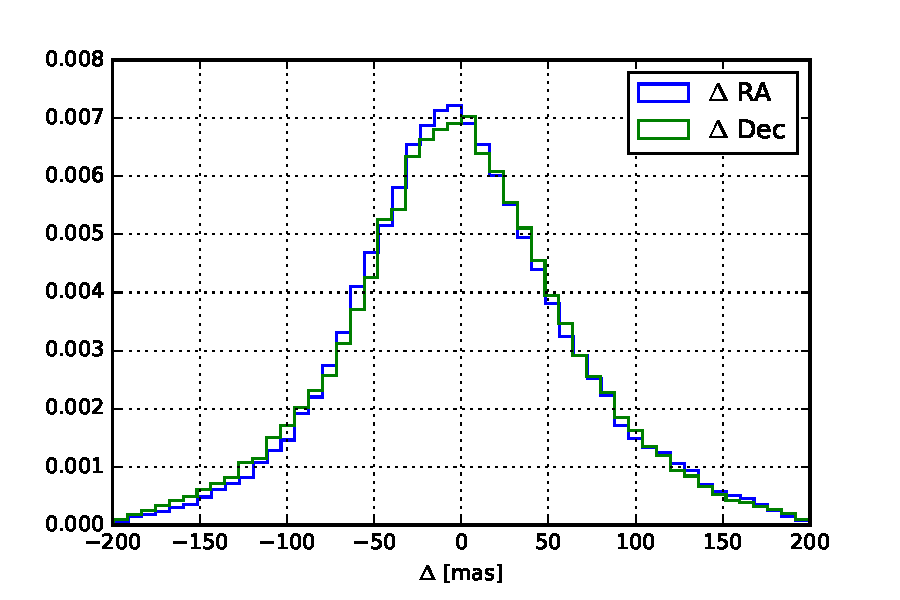
\includegraphics[width=0.45\textwidth]{astrometry_single_visit_imsim_dithered_hist}
  %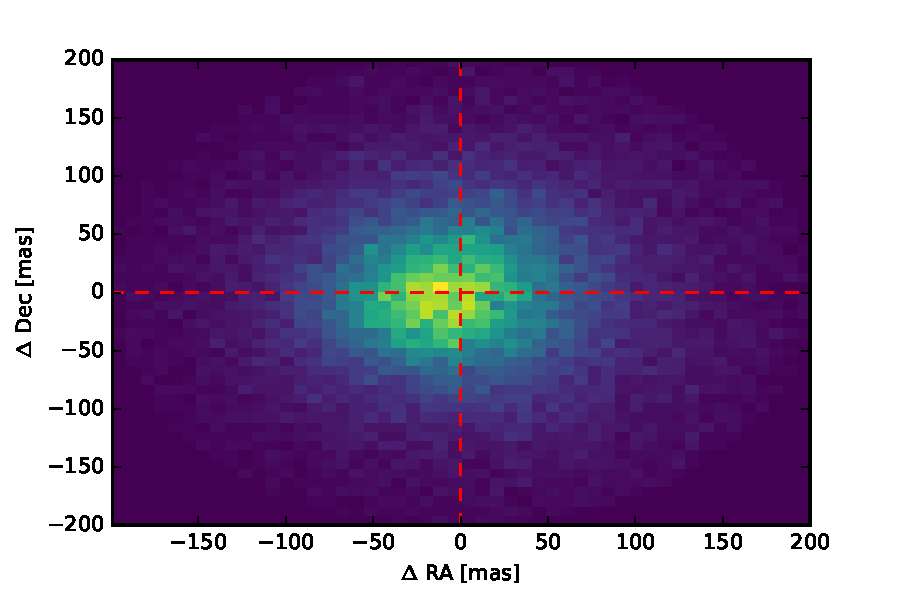
\includegraphics[width=0.45\textwidth]{astrometry_single_visit_imsim_dithered_hist2d}
  \caption{Check the per-visit depth.}
  \label{fig:depth_check_a}
\end{figure}

After this we decided to check the total depth of the coadds and its variation across the footprint. In order to do so we built
a HEALPix~\citep{2005ApJ...622..759G} map with $N_{side}=2048$ where the value in each pixel is the magnitude of the dimmest star
detected with $SNR \geq 5$. This is shown in \figref{depth_check_b} where we can see that the dithering strategy is effective and
yields a high uniformity across the footprint, especially compared with the undithered run where we can see deeper fields
in the overlap of the pointings.

\begin{figure}
  \centering
  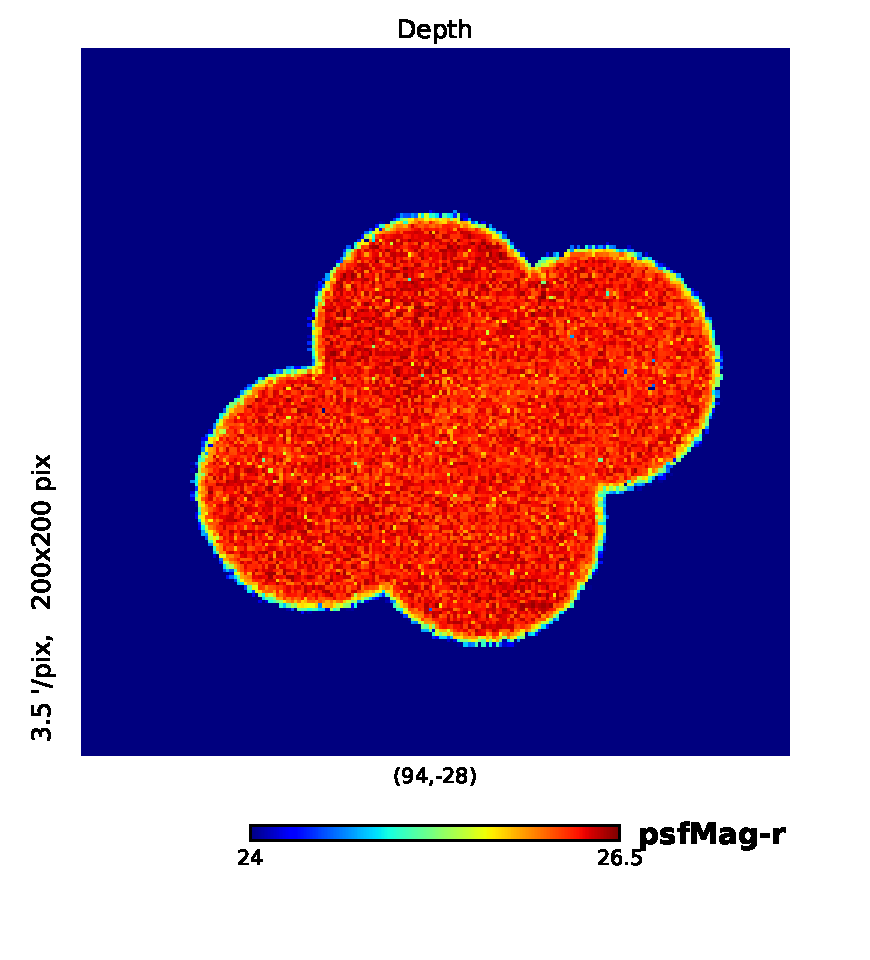
\includegraphics[width=0.3\textwidth]{depth_map_dithered}
  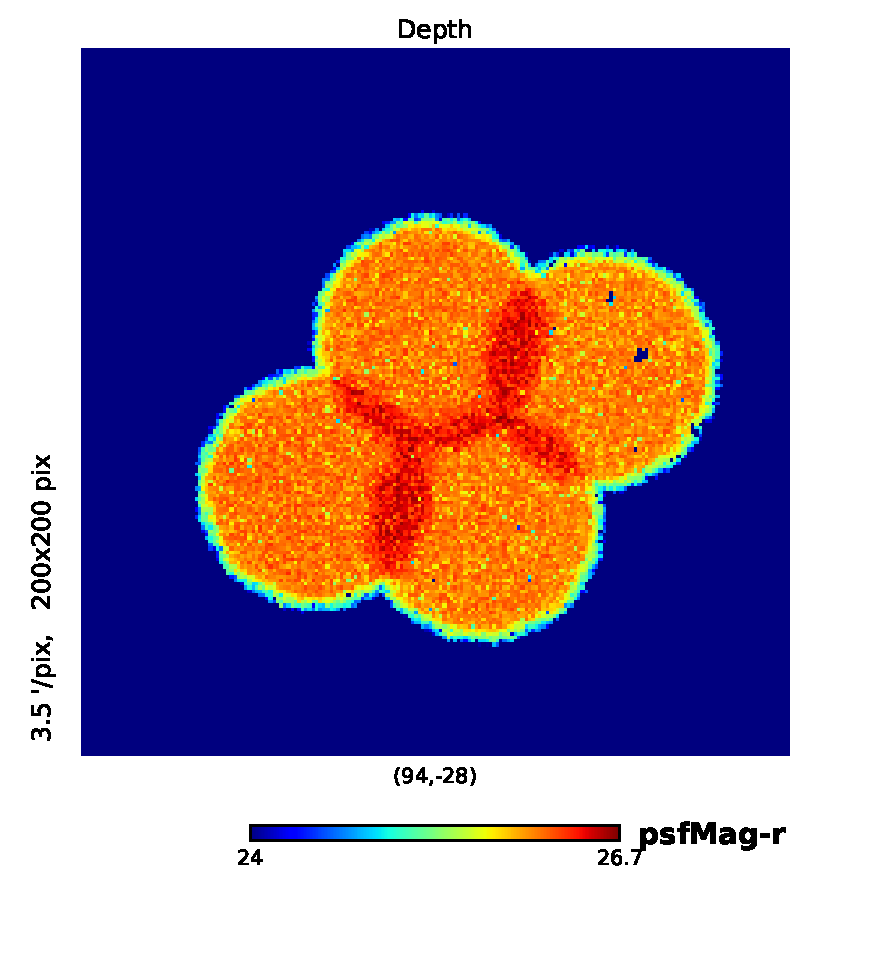
\includegraphics[width=0.3\textwidth]{depth_map_undithered}
  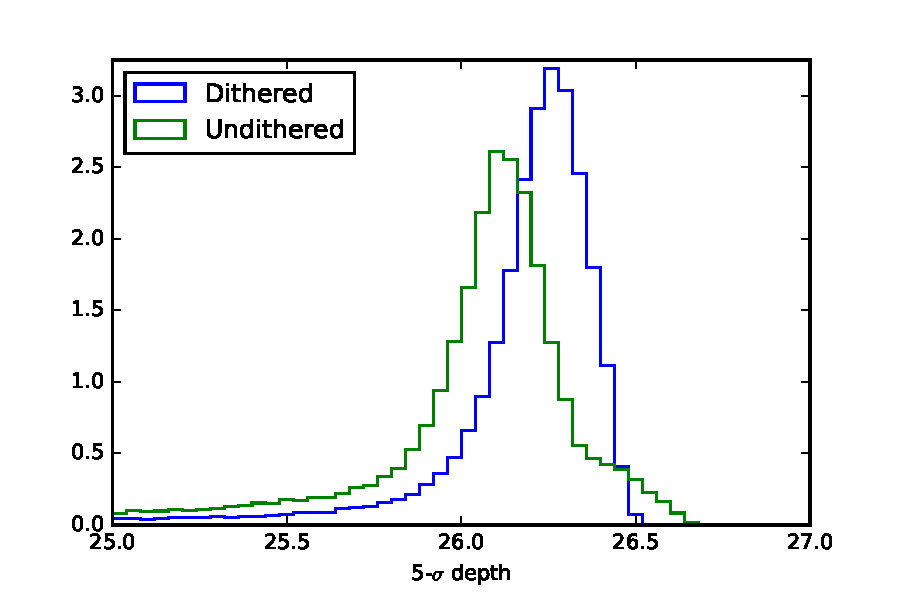
\includegraphics[width=0.3\textwidth]{5_sigma_depth_hist_imsim_dithered}
  \caption{Depth variation as a function of position in the footprint for the imSim dithered run (left) and imSim undithered run
  (center). The color scale shows the maximum PSF magnitude in each HEALPix pixel for a star detected with $SNR \geq 5$.
  We also represent the histogram showing the fraction of the area for each depth (right) for the dithered (blue) and
  undithered (green) runs. We can see that the dithering strategy results into a much uniform footprint.}
  \label{fig:depth_check_b}
\end{figure}

We also checked the density variation across the footprint as shown in \figref{fig:density_footprint}.

\begin{figure}
  \centering
  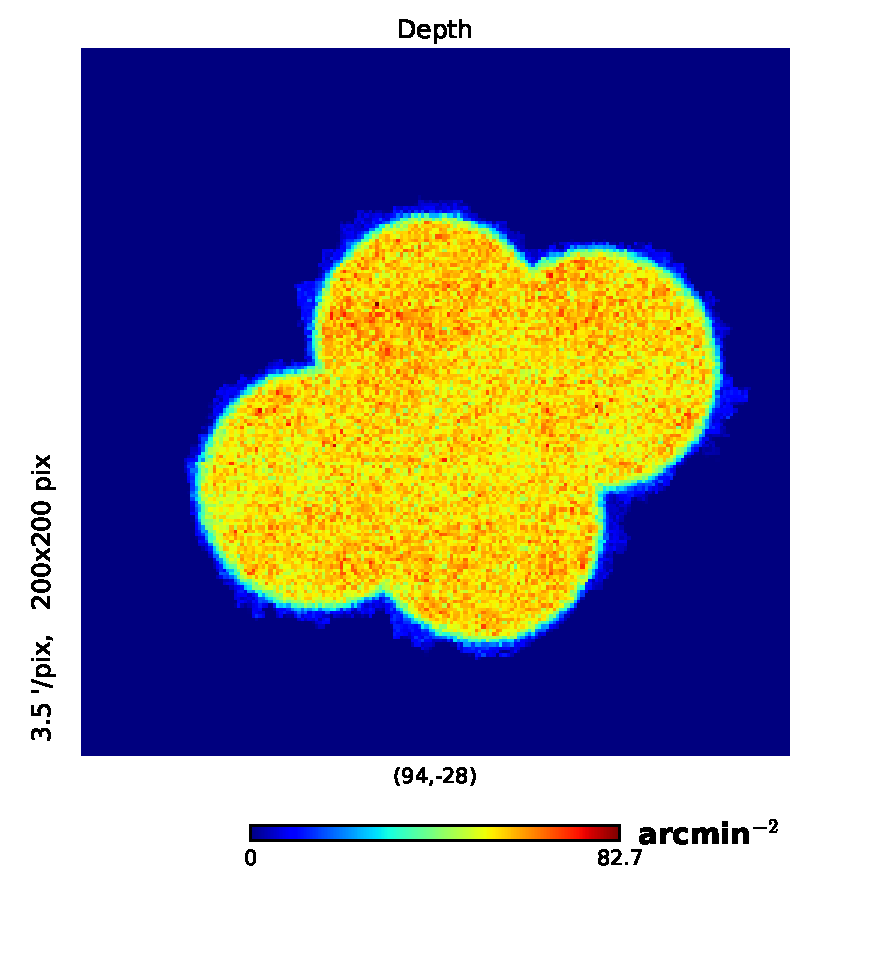
\includegraphics[width=0.45\textwidth]{density_map_dithered}
  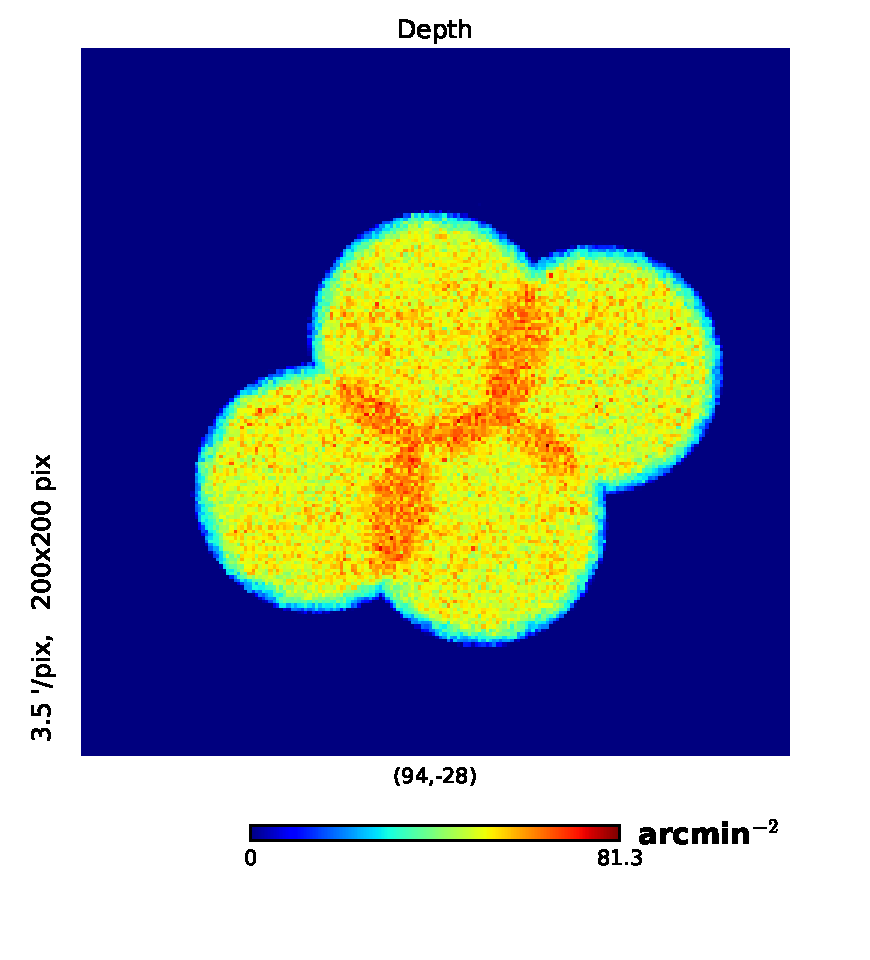
\includegraphics[width=0.45\textwidth]{density_map_undithered}
  \caption{Variation of the object density across the footprint for the imSim dithered run (left) and imSim undithered run
  (right). The color scale shows the density in units of arcmin$^{-2}$. \textcolor{red}{take out the plot's title.}}
  \label{fig:density_footprint}
\end{figure}

We focus on three different areas that can induce a systematic effect in the weak lensing and clustering observables:
astrometry, photometry and PSF.


\textcolor{red}{Add depth results and comparison with expected depth and plots with the object density.}

\subsection{Astrometry checks}
\label{sec:astrometry_checks}

Biases in astrometry can potentially affect both clustering and weak lensing measurements. These biases
can have different origins: PSF mis-characterization, non corrected sensor effects, incorrect modeling of proper
motion for the measured objects and presence of blended sources are among the most common sources.

We will follow two approaches to check the quality of the astrometric solutions that we obtained: an \textit{external} check
comparing to the input \textit{truth} catalog; and an \textit{internal} check comparing different visits.

\subsubsection{External checks}
\label{sec:external_astrometry}

As we have already mentioned, one of the big advantages of using simulations is that we have access to the \textit{true}
underlying information. We will use this information to check the precision of the astrometric measurements in single exposures
and co-adds. For these studies we will select stellar objects. In order to do so, we use the classifier
included in the LSST software stack\footnote{To see more details about the classifier refer to section 4.9.10 at
~\citep{2017arXiv170506766B}} and choose objects with \texttt{base\_ClassificationExtendedness\_value==0}.
We also require that \texttt{deblend\_nChild==0} to ensure that the objects are completely deblended, i.e., they are primary
sources. We match these objects to the stellar sources in the input catalog. In both cases we will use a
\texttt{KDTree}~\citep{scikit-learn} to retrieve those objects in the input catalog that are in a radius of 0.2 arc-seconds
(one pixel) of those detected in the output catalog and select the match that is closest in magnitude. We only consider sources
which have a magnitude difference smaller than 0.02 magnitudes.

We selected a representative single visit (visit number $270675$ for the imSim dithered run) and calculated the difference
between the measured and the input positions. These are represented in \figref{astrometry_a}. We can see that both RA and Dec
distributions are compatible with each other, meaning that there are no anisotropies in the detection, as expected from the inputs.
However, we find that the distributions are assymetric and that the median is not zero. This effect is even more noticeable when we
accumulate visits as in \figref{astrometry_b}, where we accumulated the results for 50 randomly selected visits of the imSim dithered
run. This effect is also present in the dithered and undithered imSim runs and in the PhoSim run. We also checked the dependence the
mean astrometric residual with the magnitude of the objects as shown in \figref{astrometry_b} where a mild bias for the brightest
objects can be seen. This bias is smaller than 15 mas, much smaller than the resolution of the input N-body simulation. This means
that the two point clustering statistics will not be affected by this bias.
\textcolor{red}{Check origin of these biases}

\begin{figure}
  \centering
  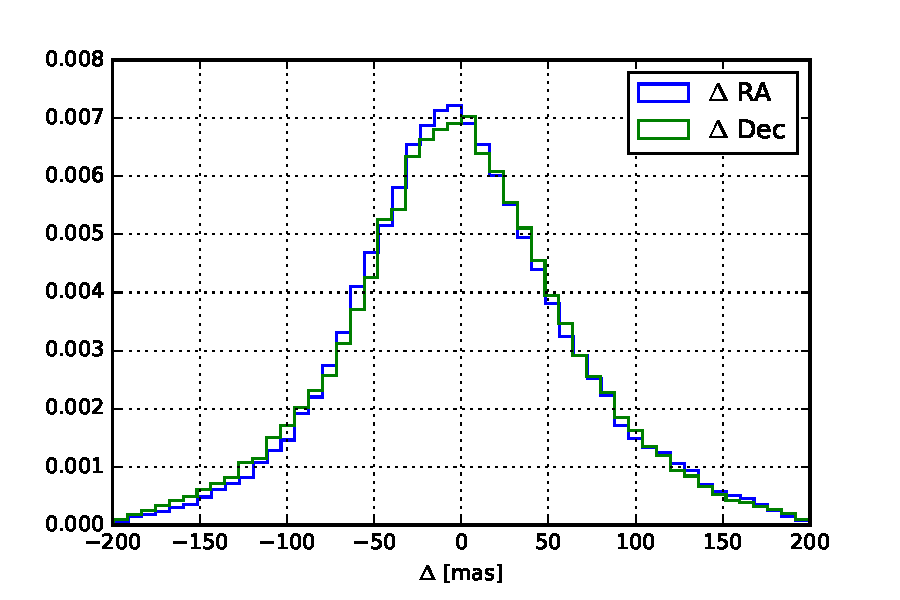
\includegraphics[width=0.45\textwidth]{astrometry_single_visit_imsim_dithered_hist}
  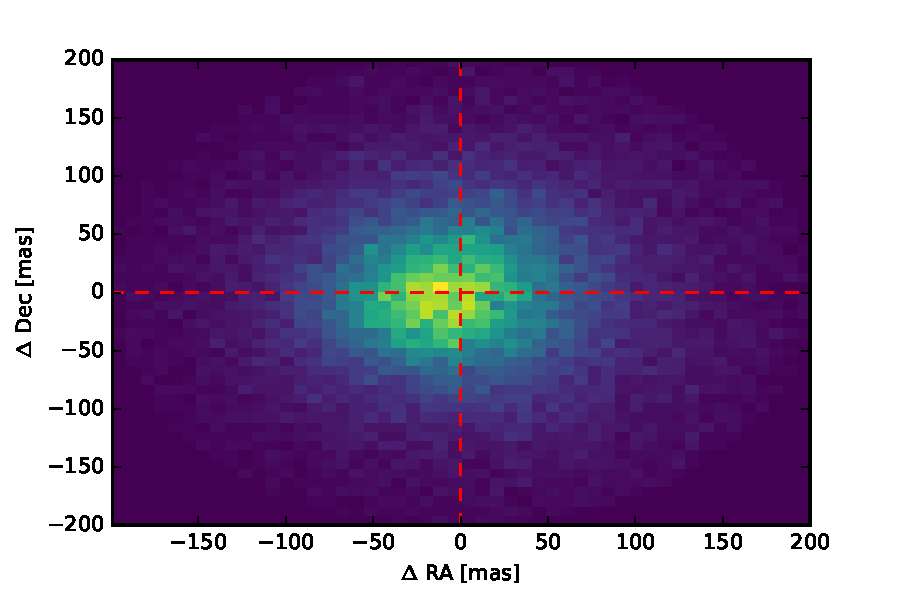
\includegraphics[width=0.45\textwidth]{astrometry_single_visit_imsim_dithered_hist2d}
  \caption{Left: Distribution of the difference $\Delta=X_{measured}-X_{input}$ in RA (blue) and Dec (green) coordinates. We cannot
  appreciate any differences between these, however we see that there is median is not at zero $\Delta_{median} \approx -2$ mas.
  The histograms are normalized such that the total sum of the counts is equal to one. Right: 2D histogram
  showing the bivariate distribution of the difference in RA (horizontal axis) and Dec (vertical axis). We selected one random representative
  exposure (visit number $270675$ for the imSim dithered run). The effect is similar for the undithered imSim run and for the PhoSim run.}
  \label{fig:astrometry_a}
\end{figure}

\begin{figure}
  \centering
  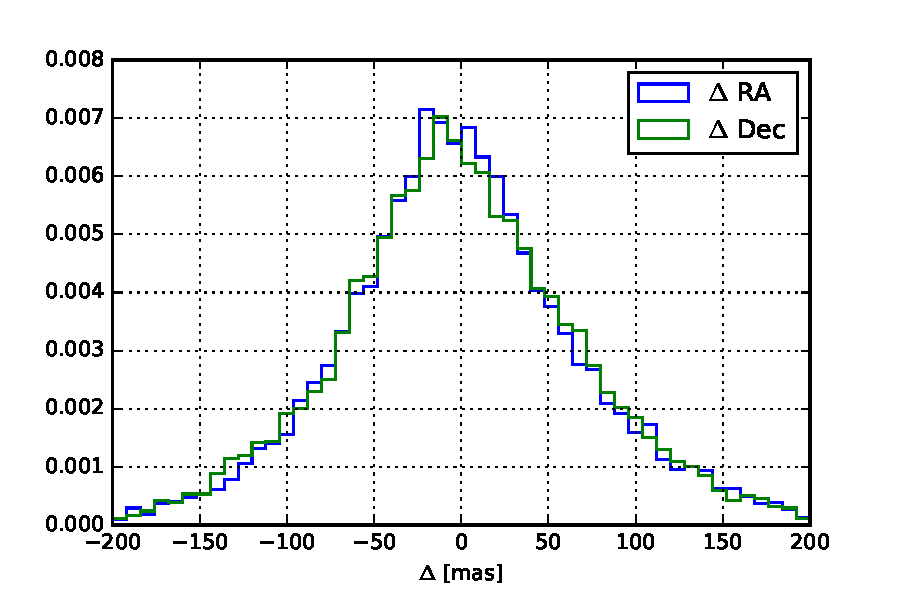
\includegraphics[width=0.3\textwidth]{astrometry_imsim_dithered_50visits}
  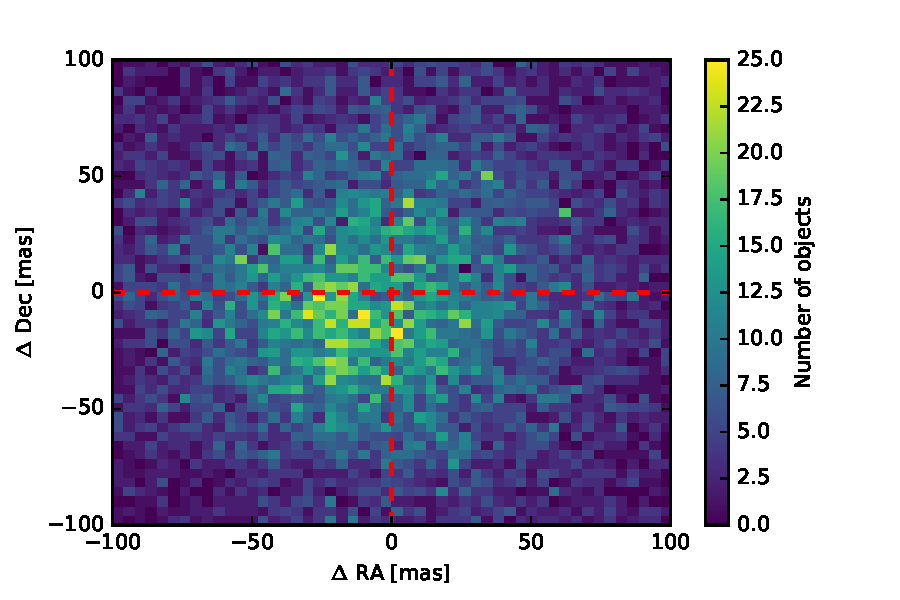
\includegraphics[width=0.3\textwidth]{astrometry_imsim_dithered_50visits_hist2d}
  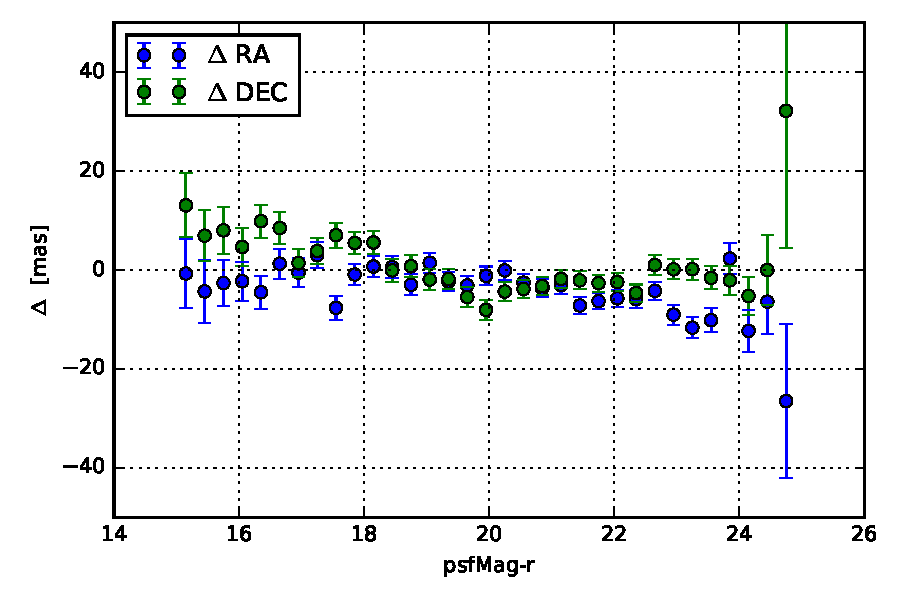
\includegraphics[width=0.3\textwidth]{astrometry_vs_mag_imsim_50_visits}
  \caption{Left: Distribution of the difference $\Delta=X_{measured}-X_{input}$ in RA (blue) and Dec (green) coordinates as in
  \figref{astrometry_a} but accumulating the results for 50 randomly selected visits from the imSim dithered run. Middle: 2D histogram
  showing the bivariate distribution of the difference in RA (horizontal axis) and Dec (vertical axis). Right: Mean astrometric residual
  as a function of magnitude for RA (blue) and Dec (green). These distributions are similar for the undithered imSim run and for the PhoSim run.}
  \label{fig:astrometry_b}
\end{figure}

We also wanted to check if there is a preferred orientation for the differences between the input and output position in a single visit. Using
the same visit as before we show the astrometric residuals in \figref{astrometry_c}. In this Figure we can see that the astrometric
residuals do not show any noticeable structure and appear to be mostly random.

\begin{figure}
  \centering
  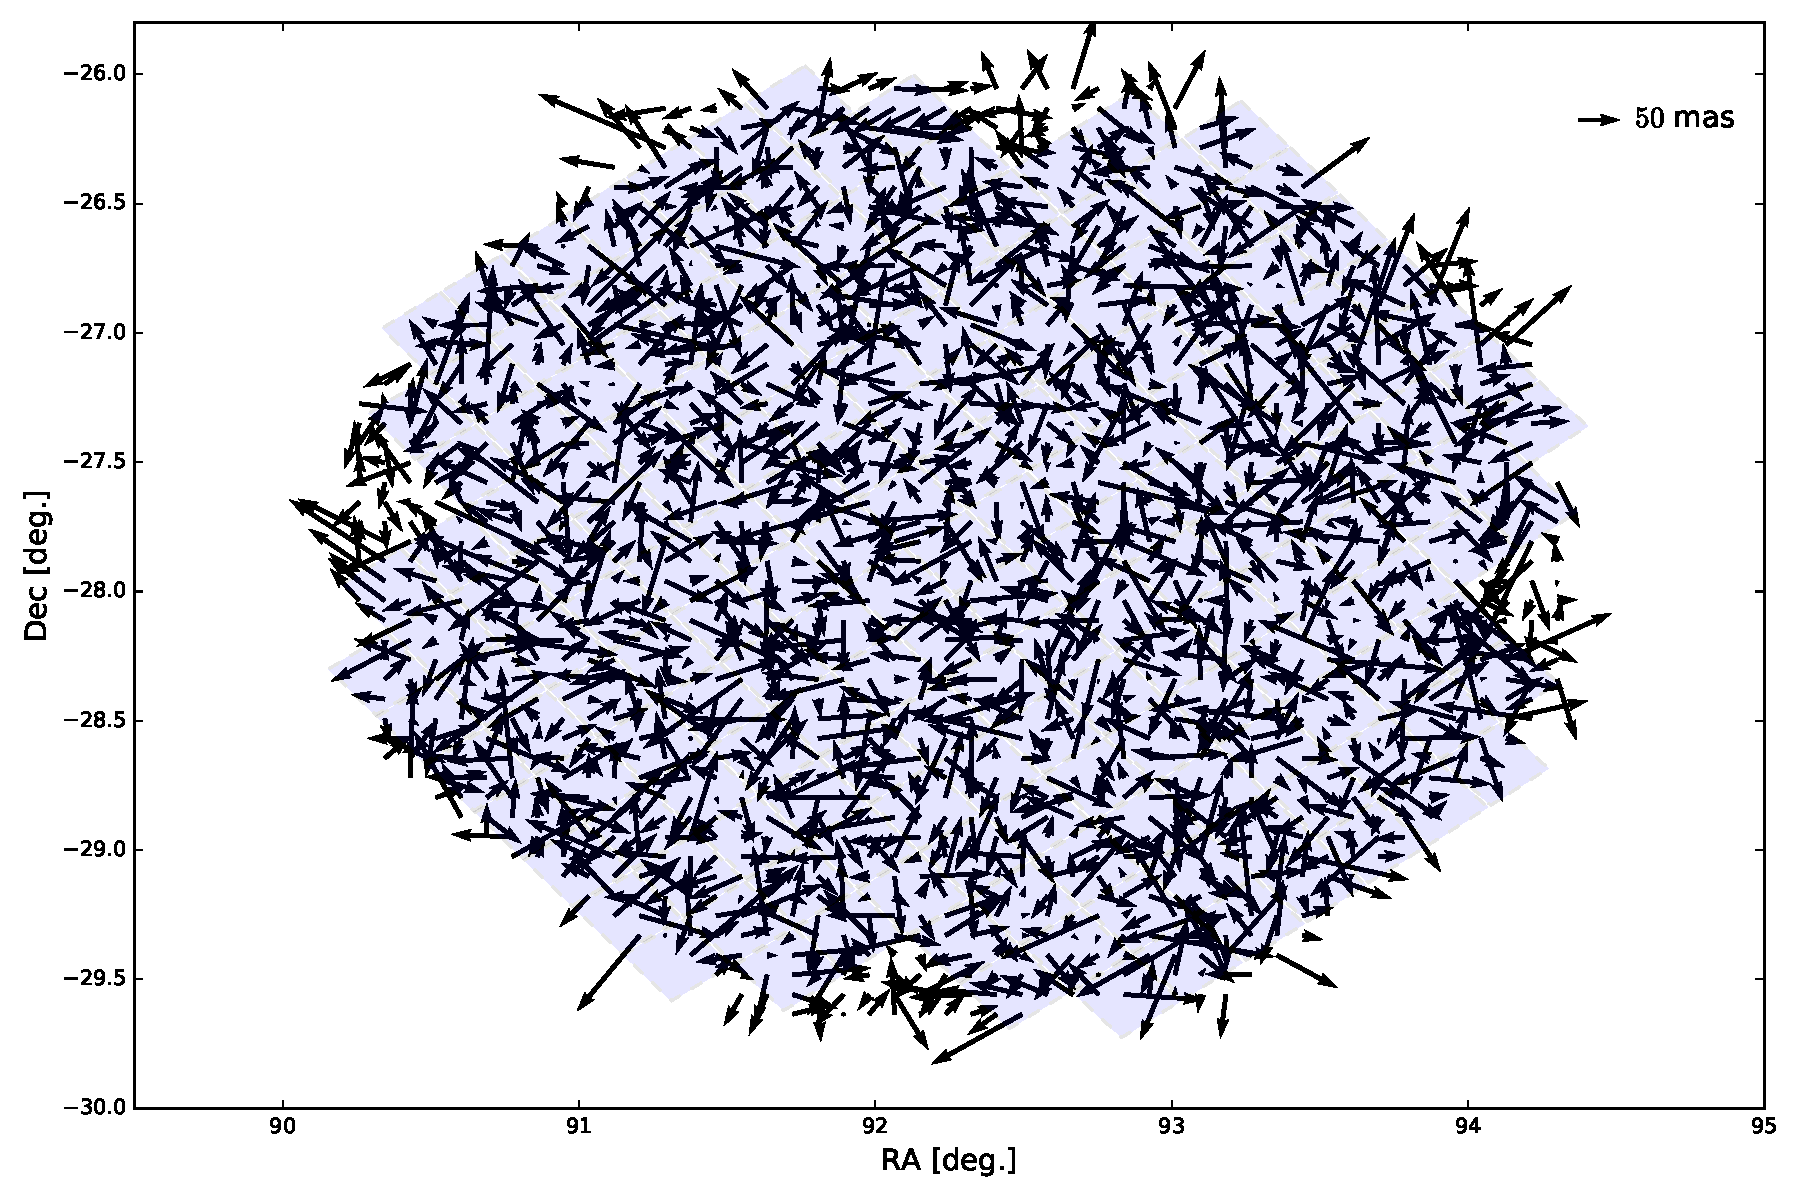
\includegraphics[width=0.7\textwidth]{astrometry_imsim_dithered_interp}
  \caption{Astrometic residuals measured in visit $270675$ from the imSim dithered run. The light blue squares represent the CCD chips in
  the LSST focal plane. The base of the arrow is on the input matched object. The arrows have been re-scaled 10,000 for visualization purposes.}
  \label{fig:astrometry_c}
\end{figure}


\subsubsection{Internal checks}
\label{sec:internal_astrometry}

Another important test is to ensure the internal consistency of the astrometric solutions between different exposures. To do that we selected
a small region of the co-added area (\textit{patch}) and compared the positions of the objects detected in the co-add
image with the positions of objects detected in individual exposures that overlap with that patch.

In particular, we randomly chose 10 catalogs from individual exposures and looked for objects that fulfilled the following criteria:
\begin{itemize}
  \item \texttt{deblend\_nChild==0}, this means that the object has been completely deblended (it is a primary match).
  \item \texttt{base\_PixelFlags\_flag\_edge==0}, which means that the object is not close to an edge.
  \item \texttt{base\_PixelFlags\_flag\_interpolatedCenter==0}, the object does not have any interpolated pixels in its center.
\end{itemize}

Note that in this case we are not requiring the objects to be clasiffied as stars (we are omitting the cut in
\texttt{base\_ClassificationExtendedness\_value}) but we are adding some cuts to ensure that the objects were properly measured. Once
we perform our selection, the next step is to match the objects in the different exposures. To do so we use the matching algorithm
included in the LSST software stack\textcolor{red}{Reference?} and calculate the mean of the difference between the position of each source
in the co-add, $X_{coadd,i}$ and the position of the matched object in each of the exposures where it has been detected, $X_{visit_{j},i}$
for $j \in [1,10]$, i.e,

\begin{equation}
  \Delta = \langle X_{coadd,i} - X_{visit_{j},i} \rangle
\end{equation}
we only consider sources that have been detected in at least 5 exposures. The resulting distribution is shown in \figref{astrometry_internal}
where we see that is noticeably narrower than those shown in \figref{astrometry_a} and \figref{astrometry_b} and no apparent bias is found showing
that the processing is consistent.

\begin{figure}
  \centering
  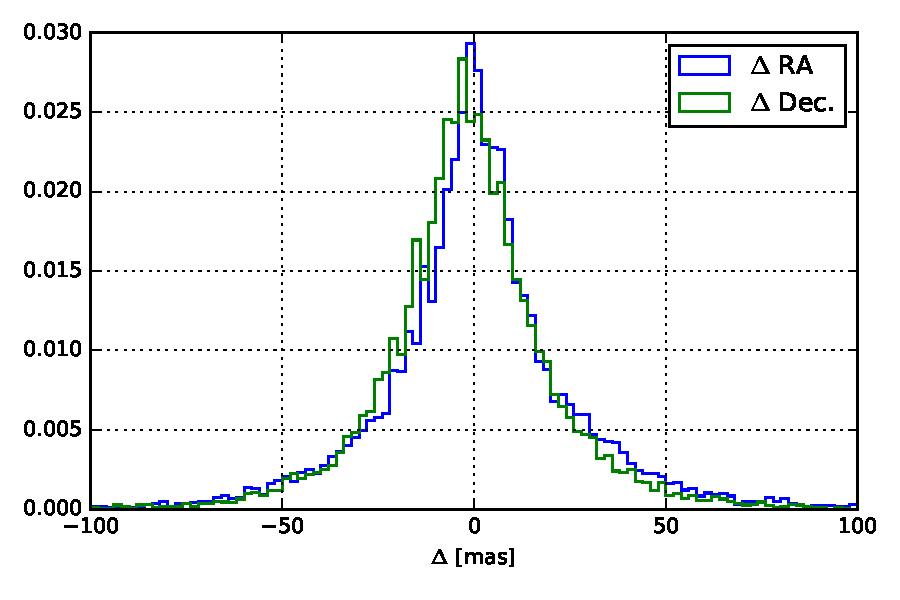
\includegraphics[width=0.45\textwidth]{astrometry_internal_10visits_imsim_undithered}
  \caption{Distribution of the mean difference in position (RA:blue, Dec:green) between the coadd and the different individual exposures
  where each source has been detected.}
  \label{fig:astrometry_internal}
\end{figure}

\subsection{Photometry checks}
\label{sec:photometry_checks}

As we did in previous sections we are going to perform two different tests to test the quality of our simulations: first we are going to
compare our output catalogs to the inputs, and second we are going to check the consistency between different visits for the same objects.

\subsubsection{External checks}
\label{sec:external_photometry}

We want to analyze the accuracy of the magnitude measurement comparing the input catalog with the output image. This process not only checks
the accuracy of the measurement pipeline but also, it tests the quality and level of realism of the image generation pipeline.
For these external checks we use again the same 50 randomly selected visits as we did in the previous section to check the astrometric residuals.
To study the photometric residuals we change slightly the matching strategy from previous sections. In this case we eliminate the threshold
in magnitude difference so, we just look for the input source that is closest in magnitude in a 0.2 arc-seconds radius around each detected
source. In \figref{photometry_a} we can see the distribution of the photometric residuals. We see that this distribution gets wider as we go
fainter (as expected) and that the 0.02 magnitude selection cut was a good proxy to ensure that we account for most sources properly matched.

\begin{figure}
  \centering
  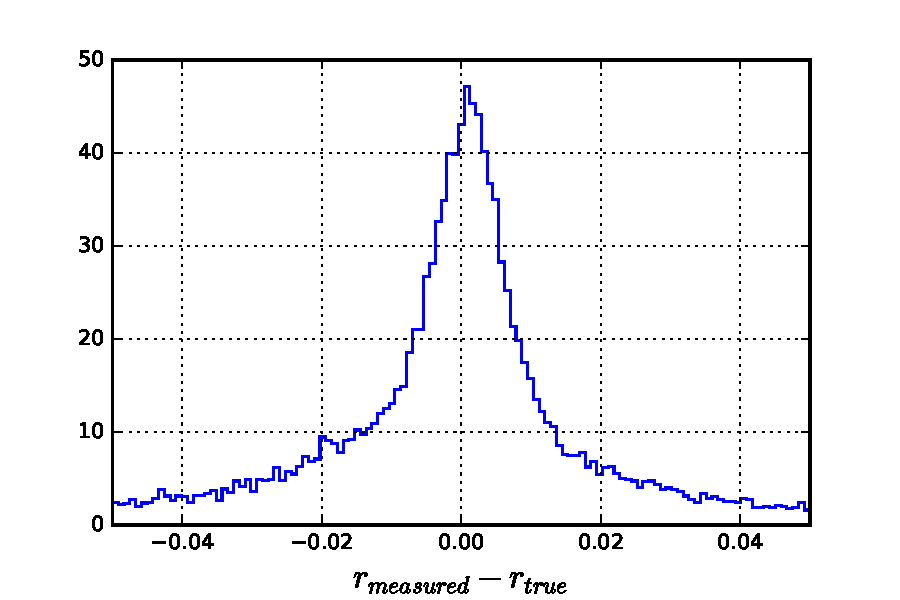
\includegraphics[width=0.45\textwidth]{photometry_imsim_dithered_50visits_hist}
  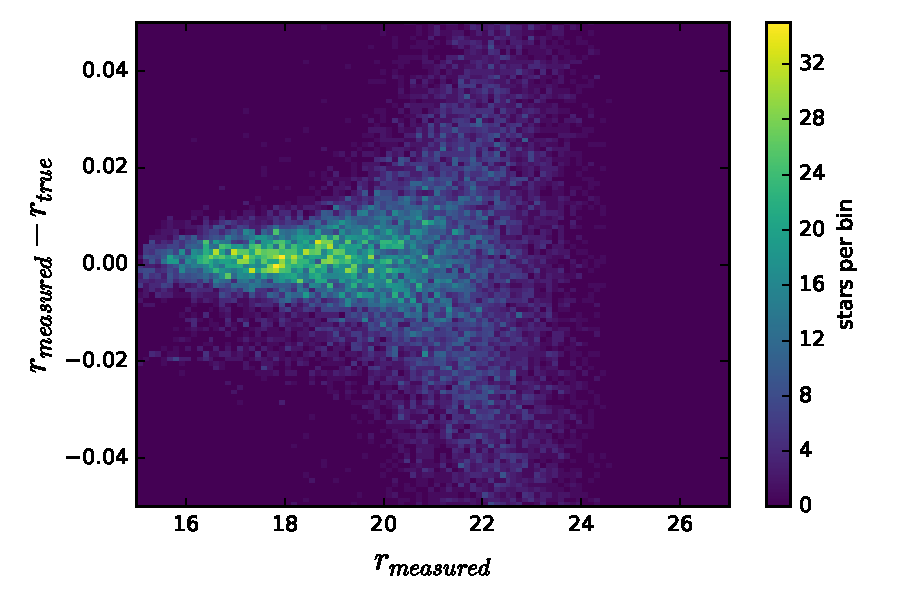
\includegraphics[width=0.45\textwidth]{photometry_imsim_dithered_50visits}
  \caption{Left: Distribution of magnitude difference between the input and output catalogs.
  Right: Difference magnitude between input and output catalogs as a function of the measured magnitude. We considered 50 visits
  randomly selected from the imSim dithered run. We find similar results for the imSim undithered run and for the PhoSim run.}
  \label{fig:photometry_a}
\end{figure}

\subsubsection{Internal checks}
\label{sec:internal_photometry}

We also checked the consistency of the photometry between different exposures. Using the same approach and sample presented in
\secref{internal_astrometry} we compared the mean difference between the coadded source and 10 random single-visit images. In
principle, we would expect that some objects will show differences between different epochs due to their intrinsic variability, however,
these effects are not found in the inputs of the simulation for any of the objects, thus, the differences between different epochs will come mainly
from statistical fluctuations and different observing conditions. The results from these checks can be seen in \figref{internal_photometry_a}.

\begin{figure}
  \centering
  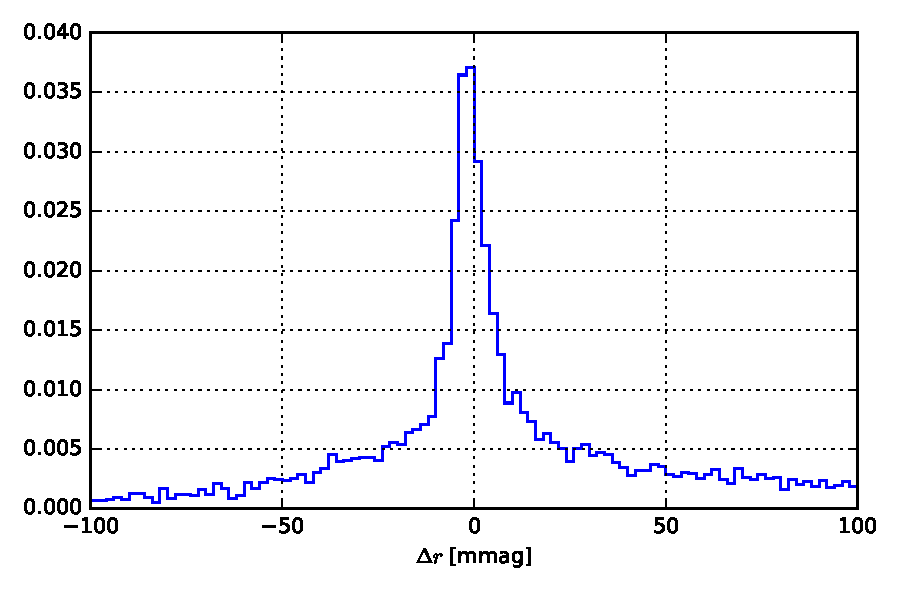
\includegraphics[width=0.45\textwidth]{photometry_internal_10visits_imsim_undithered}
  \caption{Distribution of the mean difference in magnitude between the coadd and the different individual exposures
  where each source has been detected. The mean of the distribution is consistent with zero.}
  \label{fig:internal_photometry_a}
\end{figure}

In this Figure we can see that the mean of the distribution is compatible with zero and that most sources have a magnitude difference lower
than 25 mmag given the narrow peak. However we can appreciate the presence of long tails probably due to blends and mismatching or artifacts.

\subsection{PSF checks}
\label{sec:psf_checks}

In order to ensure the accuracy of shape measurements a robust and accurate estimation of the PSF is required. In the case of imSim, we have
a perfectly known input PSF that only depends on the airmass at the time of observation. We can check if the measurement pipeline can reconstruct
the PSF and at which level of precision. To do that, we select 50 randoms visits, retrieve the measured PSF using the pipeline, and compare this
to the input model given the observing conditions and compute the residual.
% ----------------------------------------------------------------------

\section{Conclusions}
\label{sec:conclusions}

In this paper we presented the methodology followed to produce simulated images that try to resemble LSST 10-year exposures. We use two different
approaches, one based on modeling using imSim and one based on photon shooting using \textsc{PhoSim}. These two approaches are complementary
since they include different effects and also they allow us to cross-check our simulations. These images are key to investigate
the impact of systematic uncertainties in different science probes using LSST images. These images also allow us to test the image reduction and
prepare and test analysis software. This effort represents a fundamental step towards the success of LSST. We performed several tests to check the
quality and realism of the simulated products. We see that the dithered run has a high level of uniformity and points to the success of the dithering
strategy. We can also see that the PSF is recovered correctly using the pipeline.

This is the first of three different data challenges for LSST-DESC that will be increasing in complexity and size.
% ----------------------------------------------------------------------

\subsection*{Acknowledgments}

Here is where you should add your specific acknowledgments, remembering that some standard thanks will be added
via the \code{acknowledgments.tex} and \code{contributions.tex} files.

% 
This is the text imported from \code{acknowledgments.tex}, and will be replaced by some standard LSST DESC boilerplate at some point.
% 


Author contributions are listed below. \\
Yusra AlSayyad: Contribution \\
Humna Awan: Contribution \\
Colin Burke: Contribution \\
Jun Cheng: Contribution \\
James C. Chiang: Contribution \\
Scott Daniel: Contribution \\
Seth Digel: Contribution \\
Richard Dubois: Contribution \\
Eric Gawiser: Contribution \\
Tom Glanzman: Contribution \\
Mike Jarvis: Contribution \\
Tony Johnson: Contribution \\
Heather Kelly: Contribution \\
David Kirkby: Contribution \\
Simon Krughoff: Contribution \\
Robert Lupton: Contribution \\
Rachel Mandelbaum: Contribution \\
P.~Marshall: Contribution \\
Mustafa Mustafa: Contribution \\
En-Hsin Peng: Contribution \\
John Peterson: Contribution \\
Paul Price: Contribution \\
Javier Sanchez: Validation and analysis, started note \\
Glenn Sembroski: Contribution \\
Anze Slosar: Contribution \\
Brian Van Klaveren: Contribution \\
Chris W. Walter: Contribution \\
Matt Wiesener: Contribution \\
Bo Xin: Contribution \\


%{\it Facilities:} \facility{LSST}

% Include both collaboration papers and external citations:
\bibliography{lsstdesc,main}

\end{document}
% ======================================================================
%
